
\section{Results with unbalanced data}

In this section, the results are published for the experiments with the models where all the data available was used. These are all original images without any data augmentation. A total of \textbf{29966} images belonging to both the classes was used in this setup. Further details of the data distribution are presented below:

\begin{table}[H]
\centering
\begin{tabularx}{\textwidth}{@{} *4{X} @{}}
\toprule
\textbf{Label} & \textbf{Class} & \textbf{Images} & \textbf{Distribution}\\
\midrule
    Mature     & 0 & 4696 & 16\%  \\[1.3ex]
    Trout    &  1 & 25270 & 84\% \\[1.3ex]
\bottomrule
\end{tabularx}
\caption{Unbalanced dataset with all images}
\label{table:data_type1}
\end{table}


The following tables provide detailed results for two different model combination types (\ref{subsubsec:variation_1} and \ref{subsubsec:variation_2}), each associated with a specific variation. These results offer comprehensive insights into the performance and characteristics of each model within the two different model combination types. Analyzing these tables will help in understanding the impact of different architectural choices and parameter configurations on the models' performance and training duration. 

\begin{table}[H]
\centering
\begin{tabularx}{\textwidth}{@{} *5{X} @{}}
\toprule
\multicolumn{5}{c}{\textbf{Model Combination Type 1 (\ref{subsubsec:variation_1})}}                                    \\ \midrule
\raggedright \textbf{Model Metrics}           & \textbf{ResNet-50} & \textbf{MobileNet V1} & \textbf{MobileNet V2} & \textbf{MobileNet V3} \\ \midrule
Batch Size           & 32          &   64           &   64           &   64           \\ \midrule
Train Size           & 655          &  328            & 328             &  328            \\  \midrule
Validation Size      & 187          &  93            &  93            & 93             \\ \midrule
Test Size            & 95          &   47           &   47           & 47             \\ \midrule
\raggedright Total Params     &   24,637,826        &  3,754,690            &    2,914,882          &   4,883,330           \\ \midrule
\raggedright Trainable Params &   1,050,114        &  525,826            &  656,898            &   656,898           \\ \midrule
Learning Rate        &  0.001         &  0.001            &  0.001            &  0.001            \\ \midrule
Epochs               &  300         &   150           &  150            &  150            \\ \midrule
Training Time (mins)       &  301         & 86             &  87            &     88         \\ \midrule
\addlinespace
\addlinespace
\midrule
\multicolumn{5}{c}{\textbf{Model Combination Type 2 (\ref{subsubsec:variation_2})}}                                    \\ \midrule
\raggedright \textbf{Model Metrics}           & \textbf{ResNet-50} & \textbf{MobileNet V1} & \textbf{MobileNet V2} & \textbf{MobileNet V3} \\ \midrule
Batch Size           &  64          &  64            &  64            &    64          \\ \midrule
Train Size           &  328         &  328            &  328            & 328             \\  \midrule
Validation Size      &  93         &   93           &   93           & 93             \\ \midrule
Test Size            &  47         &  47            & 47             & 47             \\ \midrule
\raggedright Total Params     &  24,639,874         & 3,756,738             &  2,916,930            &  4,885,378            \\ \midrule
\raggedright Trainable Params &  1,051,138         &  526,850            &  657,922            &  657,922            \\ \midrule
Learning Rate        & 0.00001          &  0.00001            &  0.00001            &  0.00001            \\ \midrule
Epochs               & 150          &   150           &  150            &  150             \\ \midrule
Training Time (mins)       & 133          &   87           &  91            &  90             \\ \midrule
\bottomrule
\end{tabularx}
\caption{Model Setup for Combination Type 1 and 2 }
\label{table:results_1}
\end{table}


\begin{itemize}
    \item \textbf{Batch Size}: Model Combination Type 1: ResNet-50 had a batch size of 32, while MobileNet V1, V2, and V3 had a batch size of 64. Model Combination Type 2: All models had a batch size of 64.
    \item \textbf{Dataset Sizes}: Model Combination Type 1: ResNet-50 had a larger training dataset of 655 samples, while MobileNet V1, V2, and V3 used a training dataset of 328 samples. Validation and test dataset sizes were consistent across all models following a 70\%-20\%-10\% split for train, validation and test datasets. Model Combination Type 2: The dataset sizes remained consistent across all models, with 328 samples in the training dataset and 93 samples in the validation dataset and test dataset.
    \item \textbf{Total and Trainable Parameters}: Model Combination Type 1: ResNet-50 had the highest total parameters (24,637,826) and trainable parameters (1,050,114), followed by MobileNet V3, MobileNet V1, and MobileNet V2. Model Combination Type 2: ResNet-50 also had the highest total parameters (24,639,874) and trainable parameters (1,051,138), followed by MobileNet V3, MobileNet V1, and MobileNet V2.
    \item \textbf{Learning Rate and Epochs}: Model Combination Type 1: All models were trained with a learning rate of 0.001 for 150 epochs, except for ResNet-50, which was trained for 300 epochs. Model Combination Type 2: All models were trained with a learning rate of 0.00001 for 150 epochs.
    \item \textbf{Training Time}: Model Combination Type 1: ResNet-50 had the longest training time at 301 minutes, while MobileNet V1, V2, and V3 took 86-88 minutes. Model Combination Type 2: The training times ranged from 87 to 133 minutes, with MobileNet V1 having the shortest training time.

\end{itemize}


\begin{table}[H]
\centering
\begin{tabularx}{\textwidth}{@{} *5{X} @{}}
\toprule
\multicolumn{5}{c}{\textbf{Evaluation Metrics}}                                    \\ \midrule
\addlinespace
\raggedright \textbf{Metrics}           & \textbf{ResNet-50} & \textbf{MobileNet V1} & \textbf{MobileNet V2} & \textbf{MobileNet V3} \\ \midrule
\multicolumn{5}{c}{\textbf{Model Combination Type 1 (\ref{subsubsec:variation_1})}}                                    \\ \midrule
Accuracy             &  86.6\%         &  83.8\%            &  85.0\%            &  84.9\%            \\ \midrule
Precision            &  91.8\%         &  90.1\%            &  91.1\%            &  85.5\%            \\ \midrule
Recall               &  92.4\%         &  90.2\%            &  91.8\%            &  99.1\%           \\ \midrule
F1 Score               &  0.91         &  0.90            &  0.91            &  0.91           \\ \midrule
\multicolumn{5}{c}{\textbf{Model Combination Type 2 (\ref{subsubsec:variation_2})}}                                    \\ \midrule
Accuracy             &  87.0\%         &   84.9\%           &  84.9\%             &  84.8\%            \\ \midrule
Precision            &  92.4\%         &   90.9\%           &  90.8\%            &   84.8\%           \\ \midrule
Recall               &  92.3\%         &   91.3\%           &  91.6\%            &   100\%          \\ \midrule
F1 Score               &  0.92         &  0.90            &  0.90           &  0.91           \\ 
\bottomrule
\end{tabularx}
\caption{Evaluation Metrics for Model Combinations Type 1 and 2 }
\label{table:results_2}
\end{table}

Model Combination Type 1:
\begin{itemize}
    \item Accuracy ranges from 83.8\% (MobileNet V1) to 86.6\% (ResNet-50), indicating strong performance across the models.
    \item Precision scores range from 90.1\% (MobileNet V1) to 91.8\% (ResNet-50), demonstrating good ability to correctly identify positive instances.
    \item Recall scores range from 90.2\% (MobileNet V1) to 99.1\% (MobileNet V3), indicating high sensitivity in capturing positive instances.
    \item F1 scores are consistently high, ranging from 0.90 to 0.91, reflecting a balance between precision and recall.
\end{itemize}

Model Combination Type 2:

\begin{itemize}
    \item Accuracy ranges from 84.8\% (MobileNet V3) to 87.0\% (ResNet-50), showing competitive performance across the models.
    \item Precision scores range from 84.8\% (MobileNet V3) to 92.4\% (ResNet-50), indicating varying degrees of correct positive identification.
    \item Recall scores range from 91.3\% (MobileNet V2) to 100\% (MobileNet V3), demonstrating the ability to capture positive instances effectively.
    \item F1 scores range from 0.90 to 0.92, indicating a good balance between precision and recall
\end{itemize}

\subsection{ResNet-50}

\begin{figure}[H]
    \centering
    \begin{minipage}[b]{0.49\textwidth}
        \centering
        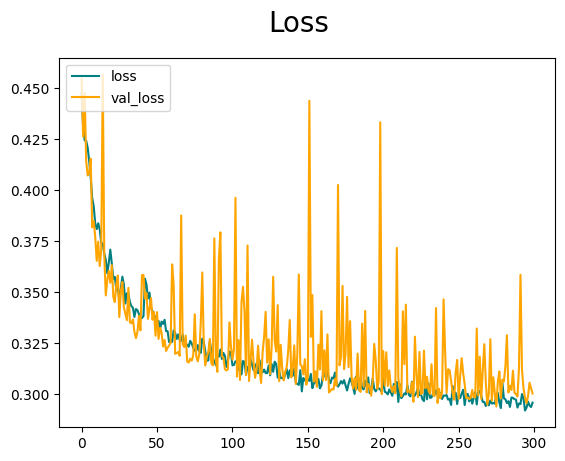
\includegraphics[width=\textwidth, height=6cm]{Figures/unbalanced_data/without bn/resnet/loss.png}
        \captionsetup{labelformat=empty}
        \caption{Combination 1}
        \label{fig:u_wo_r_l}
    \end{minipage}
    \hfill
    \begin{minipage}[b]{0.49\textwidth}
        \centering
        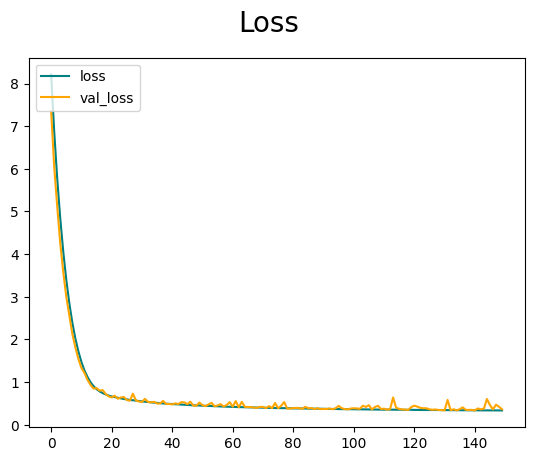
\includegraphics[width=\textwidth, height=6cm]{Figures/unbalanced_data/with bn/resnet/loss.png}
        \captionsetup{labelformat=empty}
        \caption{Combination 2}
        \label{fig:u_w_r_l}
    \end{minipage}
    \captionsetup{labelformat=default}
    \caption{ResNet-50 Loss Curves}
\end{figure}

The spikes in the validation loss in combination type 1 indicate that the model's performance on unseen data (validation set) may not be improving consistently and this can also mean that the model may be overfitting to the training data by not capturing the underlying patterns in the data effectively. It might be overly sensitive to variations or noise in the validation set, leading to inconsistent performance. As for the combination 2, we see that the loss starts at a relatively high value of 8 and decreases to less than 1 indicating that the model quickly learns and adjusts its predictions during the initial training epochs and the decreasing trend of the loss curve suggests that the model continues to improve its performance over time. The overall smoothness of the loss curve implies that the model's performance is relatively stable during training.

\begin{figure}[H]
    \centering
    \begin{minipage}[b]{0.49\textwidth}
        \centering
        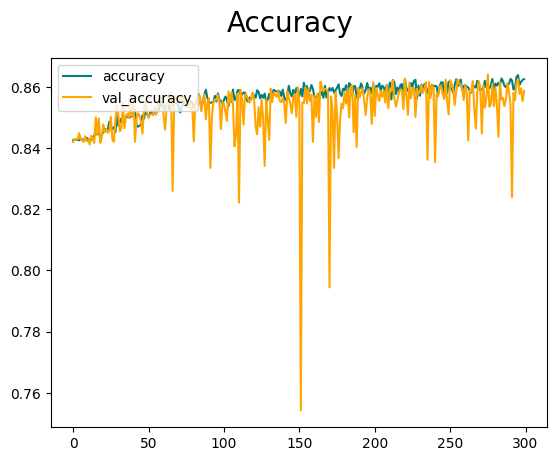
\includegraphics[width=\textwidth, height=6cm]{Figures/unbalanced_data/without bn/resnet/accuracy.png}
        \captionsetup{labelformat=empty}
        \caption{Combination 1}
        \label{fig:u_wo_r_a}
    \end{minipage}
    \hfill
    \begin{minipage}[b]{0.49\textwidth}
        \centering
        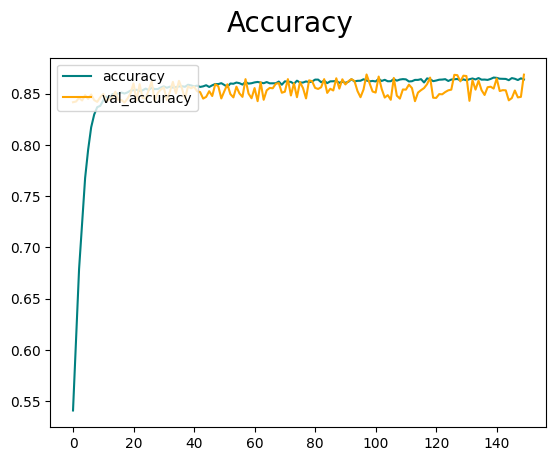
\includegraphics[width=\textwidth, height=6cm]{Figures/unbalanced_data/with bn/resnet/accuracy.png}
        \captionsetup{labelformat=empty}
        \caption{Combination 2}
        \label{fig:u_w_r_a}
    \end{minipage}
    \captionsetup{labelformat=default}
    \caption{ResNet-50 Accuracy Curves}
\end{figure}


The overall trend of the accuracy curve shows a gradual increase from around 0.84 to 0.86 over the course of 300 epochs. This suggests that the model is learning and making more accurate predictions over time. The presence of spikes in the accuracy curve indicates that there are instances where the model's performance experiences sudden drops or increases. The spikes and fluctuations in the accuracy curve may indicate that the model is encountering difficulties in converging to a stable and optimal solution. The significant drop at the 150th epoch suggests a potential setback or instability in the learning process. In the case of combination 2, the accuracy graph demonstrates notable progress, starting from a lower scale of 0.55 and reaching a range above 0.85. This suggests that the model is learning and making substantial improvements in its predictions as the training progresses. Despite the spikes in the validation curve, the fact that they remain within the range of 0.80 to 0.85 suggests a relatively consistent level of accuracy during validation. This indicates that the model is able to maintain a reasonable level of performance, although with some fluctuations.


\begin{figure}[H]
    \centering
    \begin{minipage}[b]{0.49\textwidth}
        \centering
        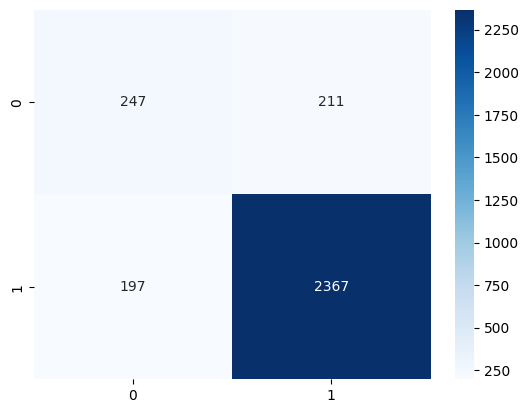
\includegraphics[width=\textwidth, height=6cm]{Figures/unbalanced_data/without bn/resnet/cm.png}
        \captionsetup{labelformat=empty}
        \caption{Combination 1}
        \label{fig:u_wo_r_cm}
    \end{minipage}
    \hfill
    \begin{minipage}[b]{0.49\textwidth}
        \centering
        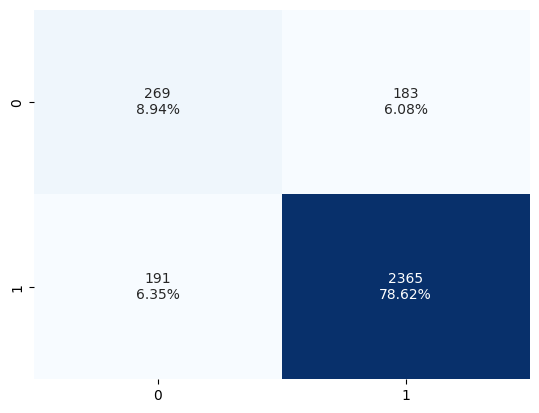
\includegraphics[width=\textwidth, height=6cm]{Figures/unbalanced_data/with bn/resnet/cm.png}
        \captionsetup{labelformat=empty}
        \caption{Combination 2}
        \label{fig:u_w_r_cm}
    \end{minipage}
    \captionsetup{labelformat=default}
    \caption{ResNet-50 Confusion Matrix}
\end{figure}

Based on the provided confusion matrices for Combination 1 and Combination 2, we can analyze the correct and wrong classification percentages for each class. \newline
For Combination 1: \textbf{Class 0 (mature)}: Correct percentage ≈ 53.95\% and the Wrong percentage ≈ 46.05\%
\textbf{Class 1 (trout)}: Correct percentage ≈ 92.29\% and the Wrong percentage ≈ 7.71\%
\newline
For Combination 2: \textbf{Class 0 (mature)}: Correct percentage ≈ 59.55\% and the Wrong percentage ≈ 40.45\%
\textbf{Class 1 (trout)}: Correct percentage ≈ 92.53\% and the Wrong percentage ≈ 7.47\%


\begin{figure}[H]
    \centering
    \begin{minipage}[b]{0.49\textwidth}
        \centering
        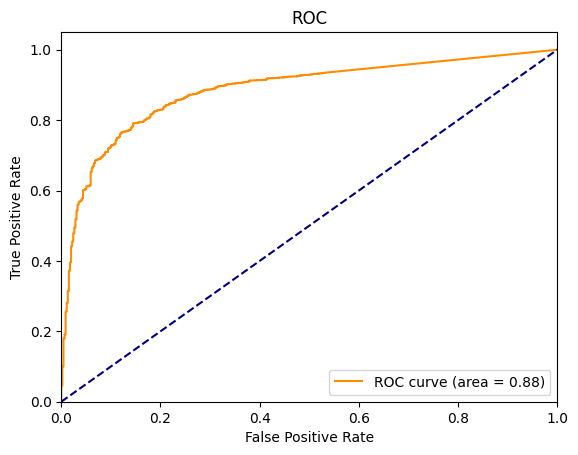
\includegraphics[width=\textwidth, height=6cm]{Figures/unbalanced_data/without bn/resnet/roc.png}
        \captionsetup{labelformat=empty}
        \caption{Combination 1}
        \label{fig:u_wo_r_roc}
    \end{minipage}
    \hfill
    \begin{minipage}[b]{0.49\textwidth}
        \centering
        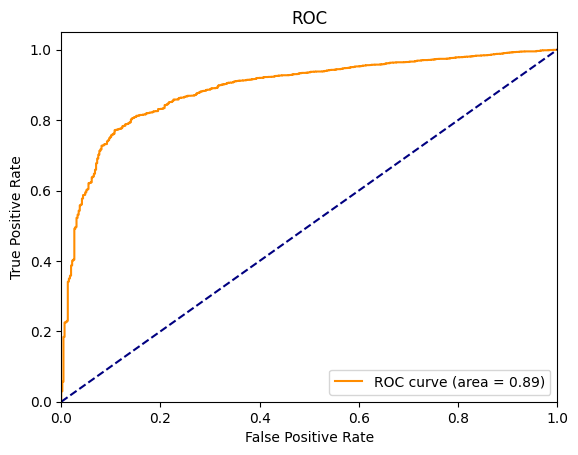
\includegraphics[width=\textwidth, height=6cm]{Figures/unbalanced_data/with bn/resnet/roc.png}
        \captionsetup{labelformat=empty}
        \caption{Combination 2}
        \label{fig:u_w_r_roc}
    \end{minipage}
    \captionsetup{labelformat=default}
    \caption{ResNet-50 Area under the ROC Curve}
\end{figure}

The AUC score ranges from 0 to 1, where a score of 0.5 indicates a random classifier and a score of 1 represents a perfect classifier. Based on the provided scores: \newline
Combination 1: AUC score = 0.88 \newline
Combination 2: AUC score = 0.89 \newline

Both the combinations have reasonably good performance in terms of their ability to discriminate between positive and negative instances.



\subsection{MobileNet V1}


\begin{figure}[H]
    \centering
    \begin{minipage}[b]{0.49\textwidth}
        \centering
        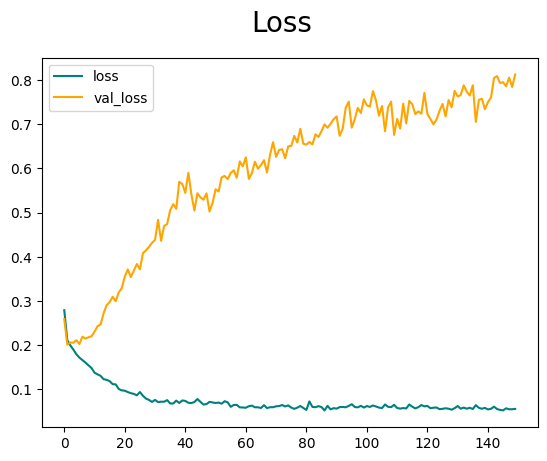
\includegraphics[width=\textwidth, height=6cm]{Figures/unbalanced_data/without bn/mn1/loss.png}
        \captionsetup{labelformat=empty}
        \caption{Combination 1}
        \label{fig:u_wo_r_l}
    \end{minipage}
    \hfill
    \begin{minipage}[b]{0.49\textwidth}
        \centering
        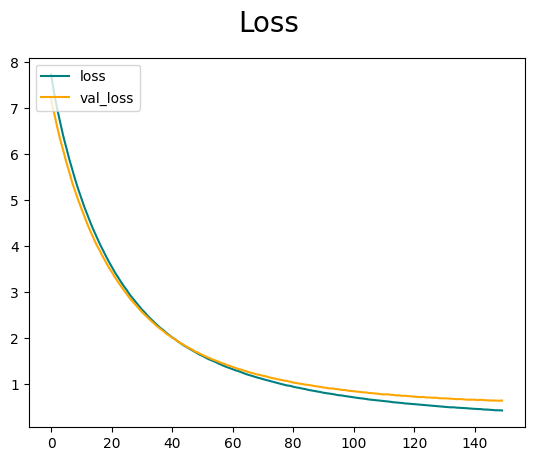
\includegraphics[width=\textwidth, height=6cm]{Figures/unbalanced_data/with bn/mn1/loss.png}
        \captionsetup{labelformat=empty}
        \caption{Combination 2}
        \label{fig:u_w_r_l}
    \end{minipage}
    \captionsetup{labelformat=default}
    \caption{MobilNet V1 Loss Curves}
\end{figure}

MobileNet V1 shows promising results in terms of train loss reduction, indicating successful learning from the training data. However, the increasing validation loss suggests a lack of generalization and potential overfitting. The validation loss curve starts at 0.3, but instead of decreasing or stabilizing, it goes up to over 0.8. This suggests that the model's performance on the validation data is not as good as on the training data. In case of combination 2, both the train and validation loss curves exhibit a smooth descent, without significant spikes or fluctuations. The validation loss curve starts at around 7 and follows a similar pattern as the train loss curve. It gradually decreases and converges around 1. This smoothness suggests that the model is consistently learning and generalizing well, without encountering major obstacles or fluctuations in performance.

\begin{figure}[H]
    \centering
    \begin{minipage}[b]{0.49\textwidth}
        \centering
        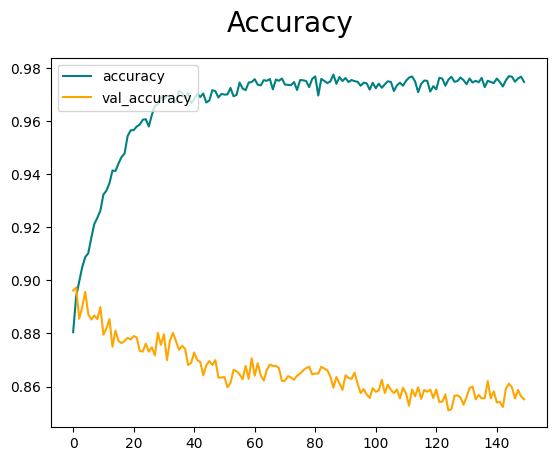
\includegraphics[width=\textwidth, height=6cm]{Figures/unbalanced_data/without bn/mn1/accuracy.png}
        \captionsetup{labelformat=empty}
        \caption{Combination 1}
        \label{fig:u_wo_r_a}
    \end{minipage}
    \hfill
    \begin{minipage}[b]{0.49\textwidth}
        \centering
        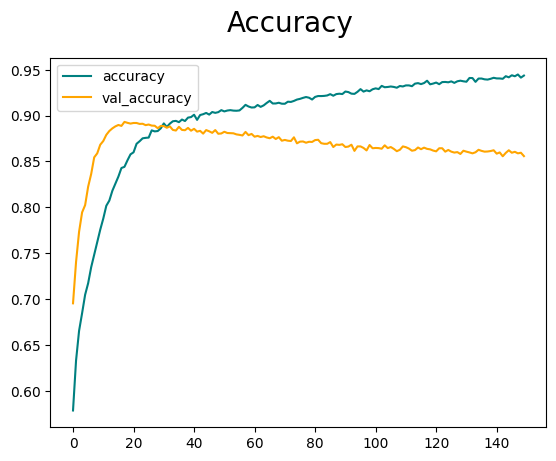
\includegraphics[width=\textwidth, height=6cm]{Figures/unbalanced_data/with bn/mn1/accuracy.png}
        \captionsetup{labelformat=empty}
        \caption{Combination 2}
        \label{fig:u_w_r_a}
    \end{minipage}
    \captionsetup{labelformat=default}
    \caption{MobilNet V1 Accuracy Curves}
\end{figure}

For Combination 1: The validation accuracy starts just below 0.9 and experiences some fluctuations with spikes during the training. It eventually settles around 0.86. While the accuracy is relatively high, the presence of spikes suggests that the model's performance on the validation data is less stable compared to the train accuracy. It indicates that the model might be overfitting to some extent and not generalizing optimally to unseen data. It demonstrates a higher train accuracy and some fluctuations in the validation accuracy, indicating potential overfitting. \newline
For Combination 2: The validation accuracy starts around 0.7 and gradually increases to a range of 0.85-0.90. It remains relatively stable within this range, indicating that the model's performance on the validation data is consistent. The consistent improvement and relatively high accuracy suggest that the model is generalizing well to unseen data. It shows a consistently improving train accuracy and a stable validation accuracy within a relatively high range.

\begin{figure}[H]
    \centering
    \begin{minipage}[b]{0.49\textwidth}
        \centering
        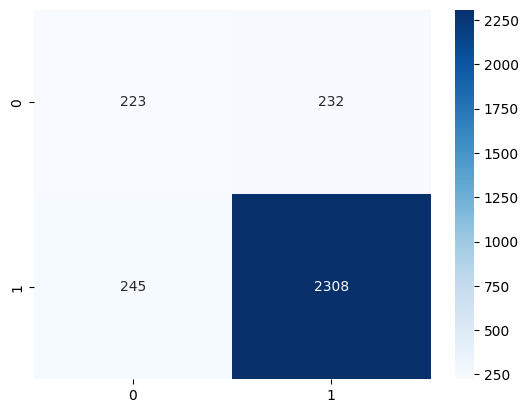
\includegraphics[width=\textwidth, height=6cm]{Figures/unbalanced_data/without bn/mn1/cm.png}
        \captionsetup{labelformat=empty}
        \caption{Combination 1}
        \label{fig:u_wo_r_cm}
    \end{minipage}
    \hfill
    \begin{minipage}[b]{0.49\textwidth}
        \centering
        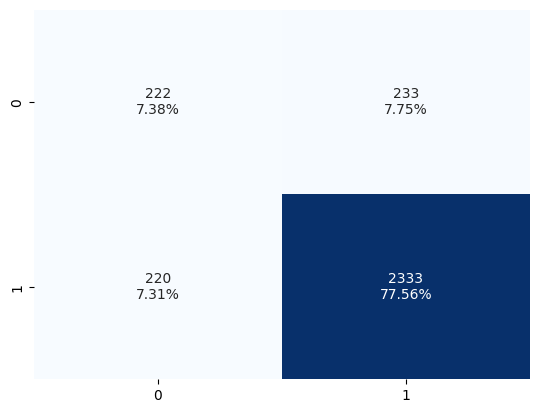
\includegraphics[width=\textwidth, height=6cm]{Figures/unbalanced_data/with bn/mn1/cm.png}
        \captionsetup{labelformat=empty}
        \caption{Combination 2}
        \label{fig:u_w_r_cm}
    \end{minipage}
    \captionsetup{labelformat=default}
    \caption{MobilNet V1 Confusion Matrix}
\end{figure}

Based on the provided confusion matrices for Combination 1 and Combination 2, we can analyze the correct and wrong classification percentages for each class. \newline
For Combination 1: \textbf{Class 0 (mature)}: Correct percentage ≈ 49.0\% and the Wrong percentage ≈ 51.0\%
\textbf{Class 1 (trout)}: Correct percentage ≈ 90.4\% and the Wrong percentage ≈ 9.6\%
\newline
For Combination 2: \textbf{Class 0 (mature)}: Correct percentage ≈ 48.8\% and the Wrong percentage ≈ 51.2\%
\textbf{Class 1 (trout)}: Correct percentage ≈ 91.4\% and the Wrong percentage ≈ 8.6\%


\begin{figure}[H]
    \centering
    \begin{minipage}[b]{0.49\textwidth}
        \centering
        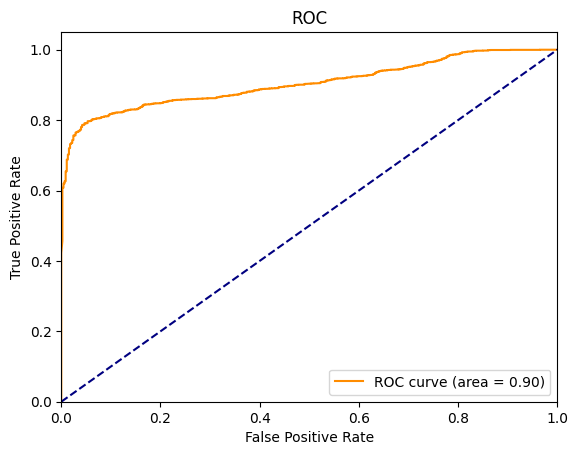
\includegraphics[width=\textwidth, height=6cm]{Figures/unbalanced_data/without bn/mn1/roc.png}
        \captionsetup{labelformat=empty}
        \caption{Combination 1}
        \label{fig:u_wo_r_roc}
    \end{minipage}
    \hfill
    \begin{minipage}[b]{0.49\textwidth}
        \centering
        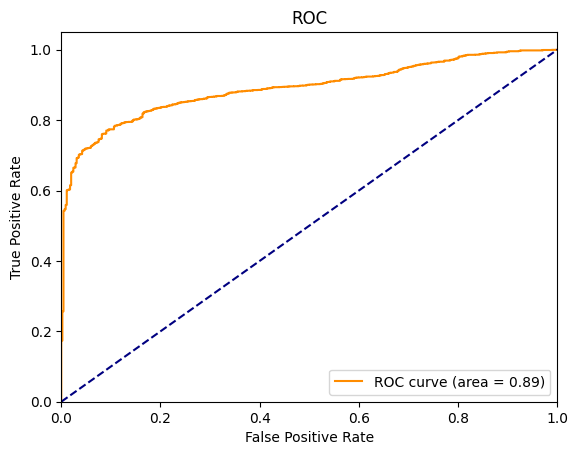
\includegraphics[width=\textwidth, height=6cm]{Figures/unbalanced_data/with bn/mn1/roc.png}
        \captionsetup{labelformat=empty}
        \caption{Combination 2}
        \label{fig:u_w_r_roc}
    \end{minipage}
    \captionsetup{labelformat=default}
    \caption{MobilNet V1 Area under the ROC Curve}
\end{figure}


The AUC score ranges from 0 to 1, where a score of 0.5 indicates a random classifier and a score of 1 represents a perfect classifier. Based on the provided scores: \newline
Combination 1: AUC score = 0.90 \newline
Combination 2: AUC score = 0.89 \newline

\subsection{MobileNet V2}

\begin{figure}[H]
    \centering
    \begin{minipage}[b]{0.49\textwidth}
        \centering
        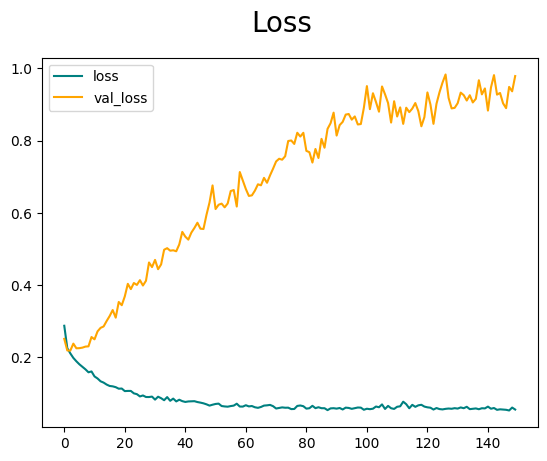
\includegraphics[width=\textwidth, height=6cm]{Figures/unbalanced_data/without bn/mn2/loss.png}
        \captionsetup{labelformat=empty}
        \caption{Combination 1}
        \label{fig:u_wo_r_l}
    \end{minipage}
    \hfill
    \begin{minipage}[b]{0.49\textwidth}
        \centering
        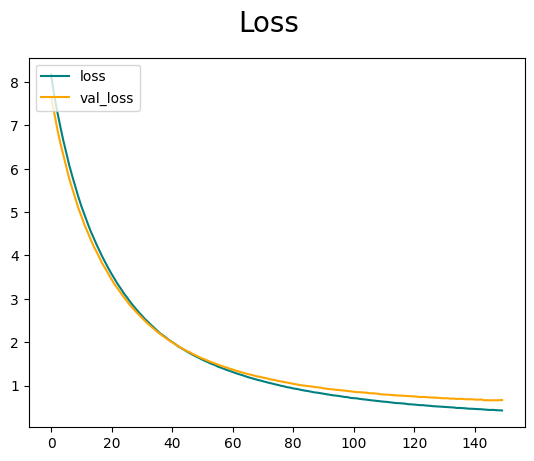
\includegraphics[width=\textwidth, height=6cm]{Figures/unbalanced_data/with bn/mn2/loss.png}
        \captionsetup{labelformat=empty}
        \caption{Combination 2}
        \label{fig:u_w_r_l}
    \end{minipage}
    \captionsetup{labelformat=default}
    \caption{MobilNet V2 Loss Curves}
\end{figure}


MobileNet V2 shows promising results in terms of train loss reduction, indicating successful learning from the training data. However, the increasing validation loss suggests a lack of generalization and potential overfitting. The validation loss curve starts just over at 0.2, but instead of decreasing or stabilizing, it goes up to around 1.0. This suggests that the model's performance on the validation data is not as good as on the training data. In case of combination 2, both the train and validation loss curves exhibit a smooth descent, without significant spikes or fluctuations. The validation loss curve starts at around 8 and follows a similar pattern as the train loss curve. It gradually decreases and converges around 1. This smoothness suggests that the model is consistently learning and generalizing well, without encountering major obstacles or fluctuations in performance.

\begin{figure}[H]
    \centering
    \begin{minipage}[b]{0.49\textwidth}
        \centering
        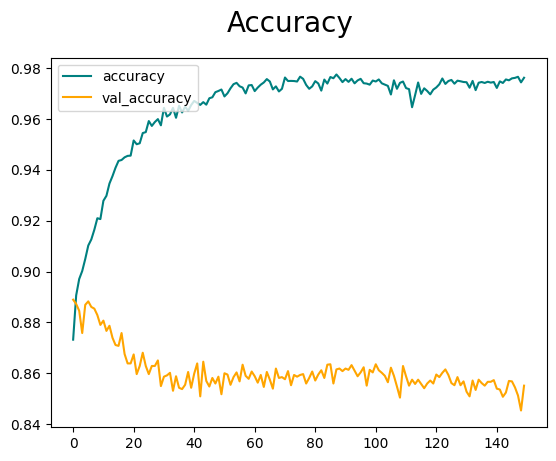
\includegraphics[width=\textwidth, height=6cm]{Figures/unbalanced_data/without bn/mn2/accuracy.png}
        \captionsetup{labelformat=empty}
        \caption{Combination 1}
        \label{fig:u_wo_r_a}
    \end{minipage}
    \hfill
    \begin{minipage}[b]{0.49\textwidth}
        \centering
        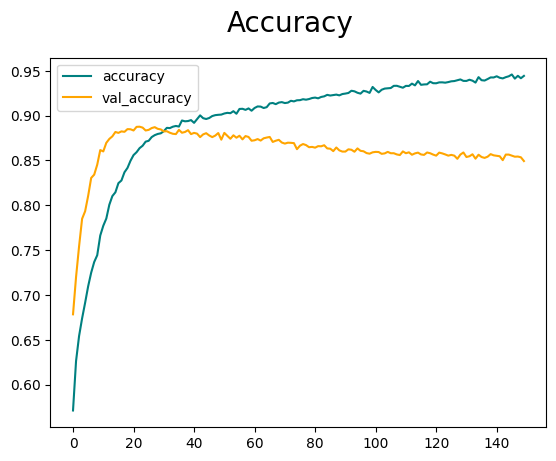
\includegraphics[width=\textwidth, height=6cm]{Figures/unbalanced_data/with bn/mn2/accuracy.png}
        \captionsetup{labelformat=empty}
        \caption{Combination 2}
        \label{fig:u_w_r_a}
    \end{minipage}
    \captionsetup{labelformat=default}
    \caption{MobilNet V2 Accuracy Curves}
\end{figure}


\begin{figure}[H]
    \centering
    \begin{minipage}[b]{0.49\textwidth}
        \centering
        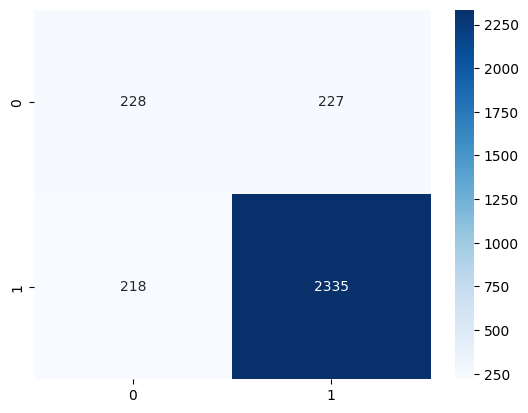
\includegraphics[width=\textwidth, height=6cm]{Figures/unbalanced_data/without bn/mn2/cm.png}
        \captionsetup{labelformat=empty}
        \caption{Combination 1}
        \label{fig:u_wo_r_cm}
    \end{minipage}
    \hfill
    \begin{minipage}[b]{0.49\textwidth}
        \centering
        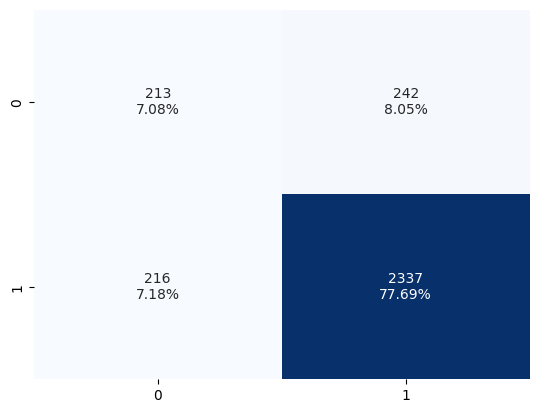
\includegraphics[width=\textwidth, height=6cm]{Figures/unbalanced_data/with bn/mn2/cm.png}
        \captionsetup{labelformat=empty}
        \caption{Combination 2}
        \label{fig:u_w_r_cm}
    \end{minipage}
    \captionsetup{labelformat=default}
    \caption{MobilNet V2 Confusion Matrix}
\end{figure}


\begin{figure}[H]
    \centering
    \begin{minipage}[b]{0.49\textwidth}
        \centering
        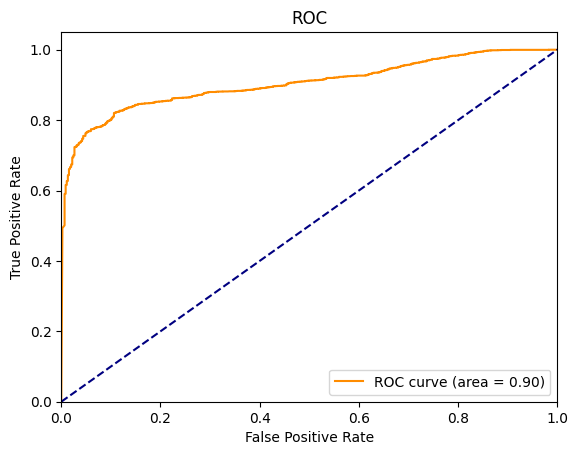
\includegraphics[width=\textwidth, height=6cm]{Figures/unbalanced_data/without bn/mn2/roc.png}
        \captionsetup{labelformat=empty}
        \caption{Combination 1}
        \label{fig:u_wo_r_roc}
    \end{minipage}
    \hfill
    \begin{minipage}[b]{0.49\textwidth}
        \centering
        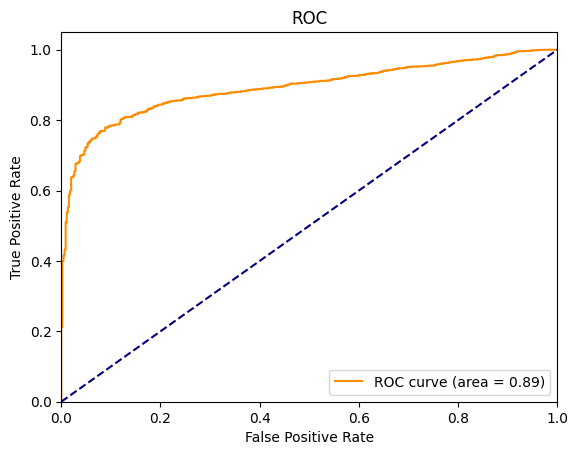
\includegraphics[width=\textwidth, height=6cm]{Figures/unbalanced_data/with bn/mn2/roc.png}
        \captionsetup{labelformat=empty}
        \caption{Combination 2}
        \label{fig:u_w_r_roc}
    \end{minipage}
    \captionsetup{labelformat=default}
    \caption{MobilNet V2 Area under the ROC Curve}
\end{figure}

\subsection{MobileNet V3}

\begin{figure}
    \centering
    \begin{subfigure}[b]{0.4\textwidth}
        \centering
        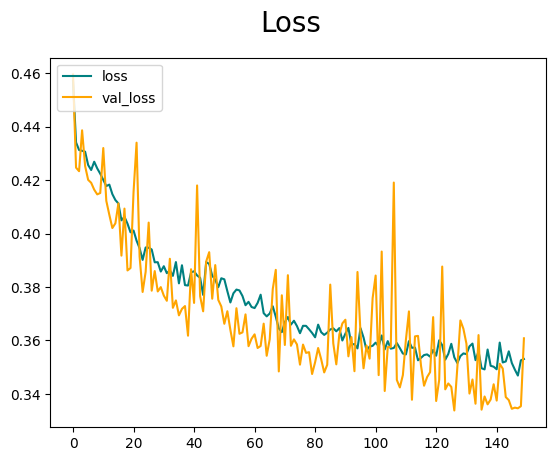
\includegraphics[width=\textwidth]{Figures/unbalanced_data/without bn/mn3/loss.png}
        \caption{Combination 1}
        \label{fig:u_wo_r_l}
    \end{subfigure}
    \begin{subfigure}[b]{0.4\textwidth}
        \centering
        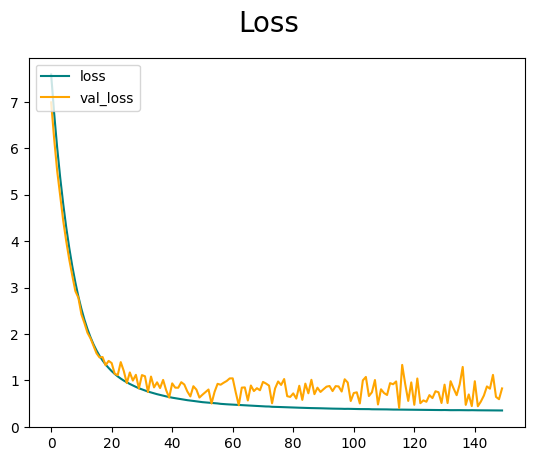
\includegraphics[width=\textwidth]{Figures/unbalanced_data/with bn/mn3/loss.png}
        \caption{Combination 2}
        \label{fig:u_w_r_l}
    \end{subfigure}
    \caption{MobilNet V3 Loss Curves}
\end{figure}

\begin{figure}[H]
    \centering
    \begin{minipage}[b]{0.49\textwidth}
        \centering
        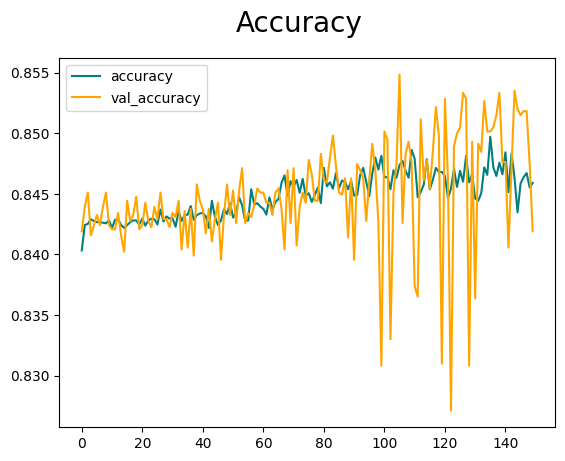
\includegraphics[width=\textwidth, height=6cm]{Figures/unbalanced_data/without bn/mn3/accuracy.png}
        \captionsetup{labelformat=empty}
        \caption{Combination 1}
        \label{fig:u_wo_r_a}
    \end{minipage}
    \hfill
    \begin{minipage}[b]{0.49\textwidth}
        \centering
        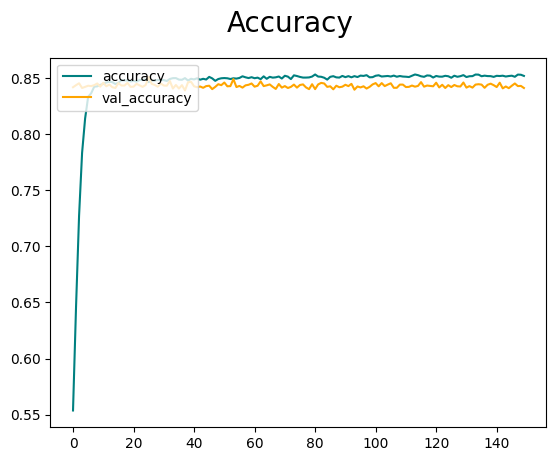
\includegraphics[width=\textwidth, height=6cm]{Figures/unbalanced_data/with bn/mn3/accuracy.png}
        \captionsetup{labelformat=empty}
        \caption{Combination 2}
        \label{fig:u_w_r_a}
    \end{minipage}
    \captionsetup{labelformat=default}
    \caption{MobilNet V3 Accuracy Curves}
\end{figure}


\begin{figure}[H]
    \centering
    \begin{minipage}[b]{0.49\textwidth}
        \centering
        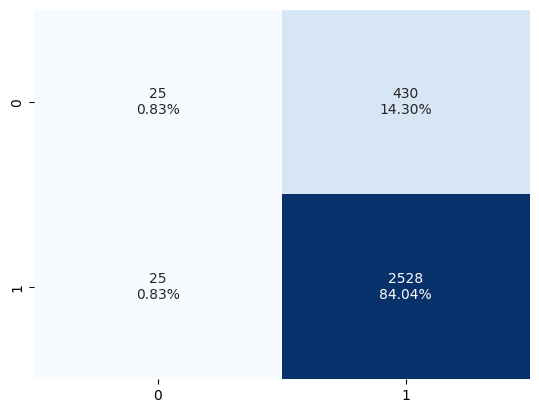
\includegraphics[width=\textwidth, height=6cm]{Figures/unbalanced_data/without bn/mn3/cm.png}
        \captionsetup{labelformat=empty}
        \caption{Combination 1}
        \label{fig:u_wo_r_cm}
    \end{minipage}
    \hfill
    \begin{minipage}[b]{0.49\textwidth}
        \centering
        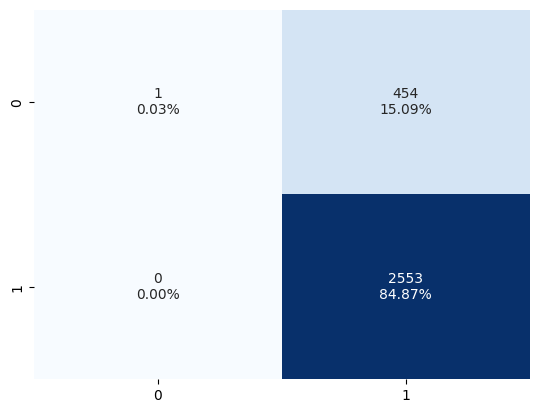
\includegraphics[width=\textwidth, height=6cm]{Figures/unbalanced_data/with bn/mn3/cm.png}
        \captionsetup{labelformat=empty}
        \caption{Combination 2}
        \label{fig:u_w_r_cm}
    \end{minipage}
    \captionsetup{labelformat=default}
    \caption{MobilNet V3 Confusion Matrix}
\end{figure}


\begin{figure}[H]
    \centering
    \begin{minipage}[b]{0.49\textwidth}
        \centering
        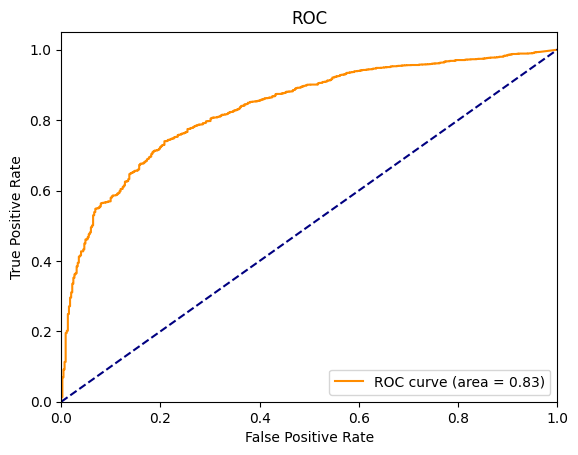
\includegraphics[width=\textwidth, height=6cm]{Figures/unbalanced_data/without bn/mn3/roc.png}
        \captionsetup{labelformat=empty}
        \caption{Combination 1}
        \label{fig:u_wo_r_roc}
    \end{minipage}
    \hfill
    \begin{minipage}[b]{0.49\textwidth}
        \centering
        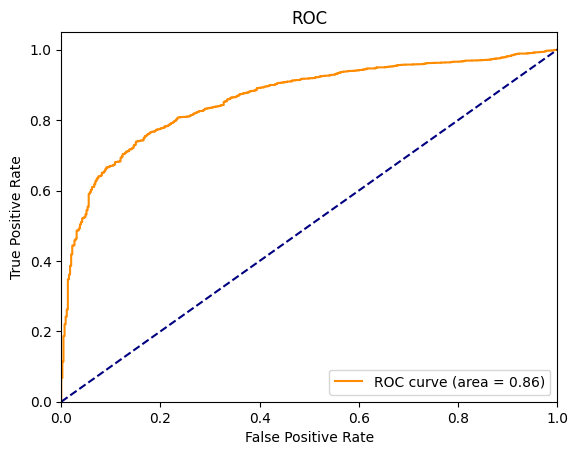
\includegraphics[width=\textwidth, height=6cm]{Figures/unbalanced_data/with bn/mn3/roc.png}
        \captionsetup{labelformat=empty}
        \caption{Combination 2}
        \label{fig:u_w_r_roc}
    \end{minipage}
    \captionsetup{labelformat=default}
    \caption{MobilNet V3 Area under the ROC Curve}
\end{figure}

\section{Results with Balanced Data}

\subsection{Without Augmentation}

\begin{table}[H]
\centering
\begin{tabularx}{\textwidth}{@{} *4{X} @{}}
\toprule
\textbf{Label} & \textbf{Class} & \textbf{Images} & \textbf{Distribution}\\
\midrule
    Mature     & 0 & 4696 & 49\%  \\[1.3ex]
    Trout    &  1 & 5000 & 51\% \\[1.3ex]
\bottomrule
\end{tabularx}
\caption{Balanced dataset with less images}
\label{table:data_type2}
\end{table}


\begin{table}[H]
\centering
\begin{tabularx}{\textwidth}{@{} *5{X} @{}}
\toprule
\multicolumn{5}{c}{\textbf{Model Variation Type 1 (\ref{subsubsec:variation_1})}}                                    \\ \midrule
\raggedright \textbf{Model Metrics}           & \textbf{ResNet-50}    & \textbf{MobileNet V1} & \textbf{MobileNet V2} & \textbf{MobileNet V3 Large} \\ \midrule
Batch Size                      &  64             & 64                &   64           &   64            \\ \midrule
Train Size                      & 106             &  106              &   106          &   106             \\  \midrule
Validation Size                 & 30              & 30                &   30           &   30            \\ \midrule
Test Size                       & 16              &  16               &   16           &   16            \\ \midrule
\raggedright Total Params       &  24,637,826     & 3,754,690         &   2,914,882    &   4,883,330                   \\ \midrule
\raggedright Trainable Params   &  1,050,114      & 525,826           &   656,898      &   656,898           \\ \midrule
Learning Rate                   & 0.001           & 0.001             &   0.001        &   0.001           \\ \midrule
Epochs                          &  150            & 150               &   150          &   150           \\ \midrule
Training Time (mins)            &  48             & 28                &   32           &   32           \\ \midrule
\addlinespace
\addlinespace
\midrule
\multicolumn{5}{c}{\textbf{Model Variation Type 2 (\ref{subsubsec:variation_2})}}                                    \\ \midrule
\raggedright \textbf{Model Metrics}           & \textbf{ResNet-50} & \textbf{MobileNet V1} & \textbf{MobileNet V2} & \textbf{MobileNet V3} \\ \midrule
Batch Size           &  64                    &  64             &  64               &   64           \\ \midrule
Train Size           &  106                   & 106             &  106              &   106               \\  \midrule
Validation Size      &  30                      &  30            &  30              &   30           \\ \midrule
Test Size            &  16                      &  16            &  16              &   16           \\ \midrule
\raggedright Total Params     & 24,639,874      &  3,756,738            & 2,916,930 &   4,885,378           \\ \midrule
\raggedright Trainable Params & 1,051,138       & 526,850             &  657,922    &   657,922           \\ \midrule
Learning Rate        &  0.00001                 & 0.00001             &  0.00001    &   0.00001           \\ \midrule
Epochs               &  150                     & 150             &  150            &   150           \\ \midrule
Training Time (mins)        &  50               & 28             &   32             &   32           \\ \midrule
\bottomrule
\end{tabularx}
\caption{Model Setup for Combination Type 1 and 2 }
\label{table:results_3}
\end{table}


\begin{table}[H]
\centering
\begin{tabularx}{\textwidth}{@{} *5{X} @{}}
\toprule
\multicolumn{5}{c}{\textbf{Evaluation Metrics}}                                    \\ \midrule
\addlinespace
\raggedright \textbf{Metrics}           & \textbf{ResNet-50} & \textbf{MobileNet V1} & \textbf{MobileNet V2} & \textbf{MobileNet V3} \\ \midrule
\multicolumn{5}{c}{\textbf{Model Combination Type 1 (\ref{subsubsec:variation_1})}}                                    \\ \midrule
Accuracy                        &  76.2\%         & 82.5\%            &   82.6\%       &   71.5\%           \\ \midrule
Precision                       &  72.8\%         & 85.7\%            &   86.5\%       &   68.8\%           \\ \midrule
Recall                          &  87.8\%         & 80.3\%            &   79.6\%       &   84.5\%          \\ \midrule
F1 Score               &  0.79         &  0.82            &  0.82            & 0.75           \\ \midrule
\multicolumn{5}{c}{\textbf{Model Combination Type 2 (\ref{subsubsec:variation_2})}}                                    \\ \midrule
Accuracy             &  72.9\%                  &   85.9\%           &  83.7\%      &   53.8\%           \\ \midrule
Precision            &  69.1\%                  &   87.4\%           &  85.4\%      &   53.4\%           \\ \midrule
Recall               &  88.9\%                  &   85.9\%           &  83.3\%      &   99.4\%          \\ \midrule
F1 Score               &  0.77         &  0.86            &  0.84            &   0.69         \\ 
\bottomrule
\end{tabularx}
\caption{Evaluation Metrics for Model Combinations Type 1 and 2 }
\label{table:results_4}
\end{table}

\subsubsection{ResNet-50}

\begin{figure}[H]
    \centering
    \begin{minipage}[b]{0.49\textwidth}
        \centering
        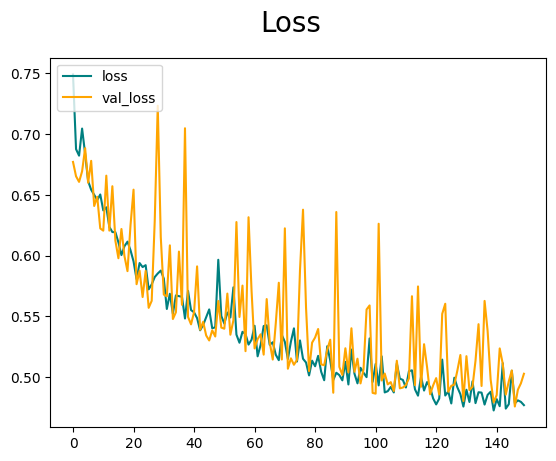
\includegraphics[width=\textwidth, height=6cm]{Figures/balanced_data/less_data/withoutbn/resnet/loss.png}
        \captionsetup{labelformat=empty}
        \caption{Combination 1}
        \label{fig:u_wo_r_l}
    \end{minipage}
    \hfill
    \begin{minipage}[b]{0.49\textwidth}
        \centering
        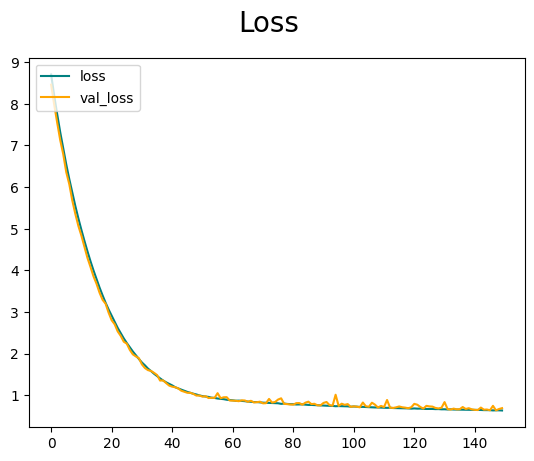
\includegraphics[width=\textwidth, height=6cm]{Figures/balanced_data/less_data/withbn/resnet/loss.png}
        \captionsetup{labelformat=empty}
        \caption{Combination 2}
        \label{fig:u_w_r_l}
    \end{minipage}
    \captionsetup{labelformat=default}
    \caption{ResNet-50 Loss Curves}
\end{figure}

\begin{figure}[H]
    \centering
    \begin{minipage}[b]{0.49\textwidth}
        \centering
        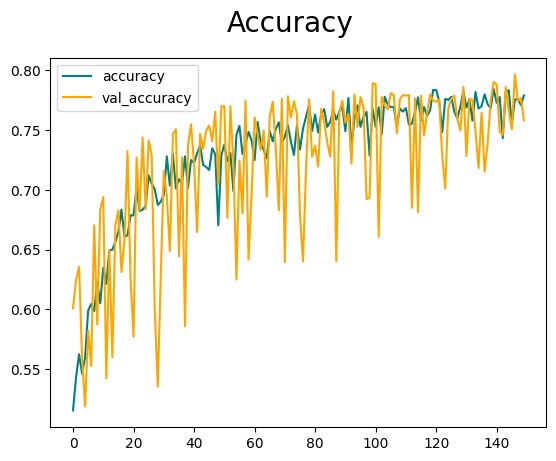
\includegraphics[width=\textwidth, height=6cm]{Figures/balanced_data/less_data/withoutbn/resnet/accuracy.png}
        \captionsetup{labelformat=empty}
        \caption{Combination 1}
        \label{fig:u_wo_r_a}
    \end{minipage}
    \hfill
    \begin{minipage}[b]{0.49\textwidth}
        \centering
        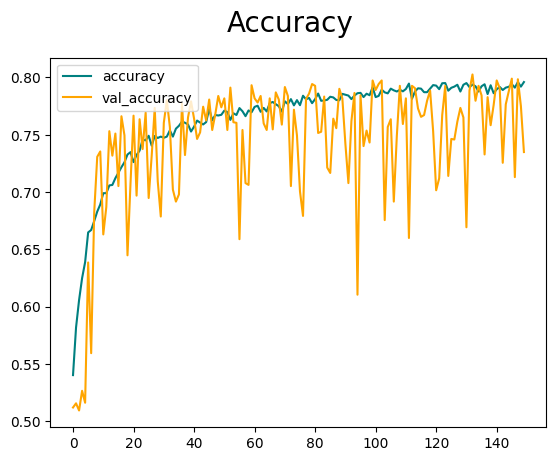
\includegraphics[width=\textwidth, height=6cm]{Figures/balanced_data/less_data/withbn/resnet/accuracy.png}
        \captionsetup{labelformat=empty}
        \caption{Combination 2}
        \label{fig:u_w_r_a}
    \end{minipage}
    \captionsetup{labelformat=default}
    \caption{ResNet-50 Accuracy Curves}
\end{figure}


\begin{figure}[H]
    \centering
    \begin{minipage}[b]{0.49\textwidth}
        \centering
        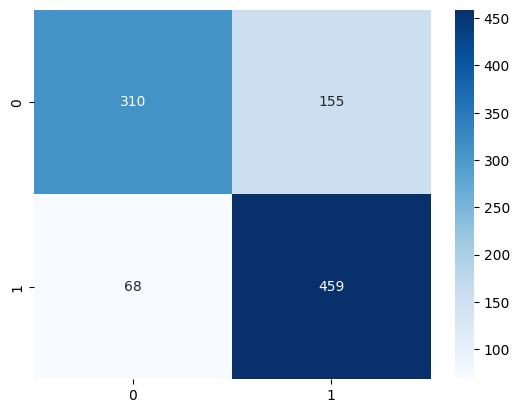
\includegraphics[width=\textwidth, height=6cm]{Figures/balanced_data/less_data/withoutbn/resnet/cm.png}
        \captionsetup{labelformat=empty}
        \caption{Combination 1}
        \label{fig:u_wo_r_cm}
    \end{minipage}
    \hfill
    \begin{minipage}[b]{0.49\textwidth}
        \centering
        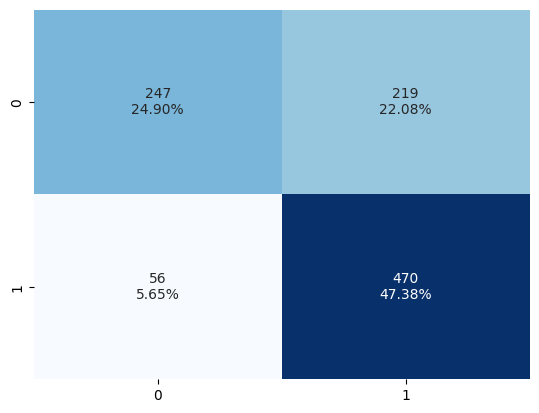
\includegraphics[width=\textwidth, height=6cm]{Figures/balanced_data/less_data/withbn/resnet/cm.png}
        \captionsetup{labelformat=empty}
        \caption{Combination 2}
        \label{fig:u_w_r_cm}
    \end{minipage}
    \captionsetup{labelformat=default}
    \caption{ResNet-50 Confusion Matrix}
\end{figure}


\begin{figure}[H]
    \centering
    \begin{minipage}[b]{0.49\textwidth}
        \centering
        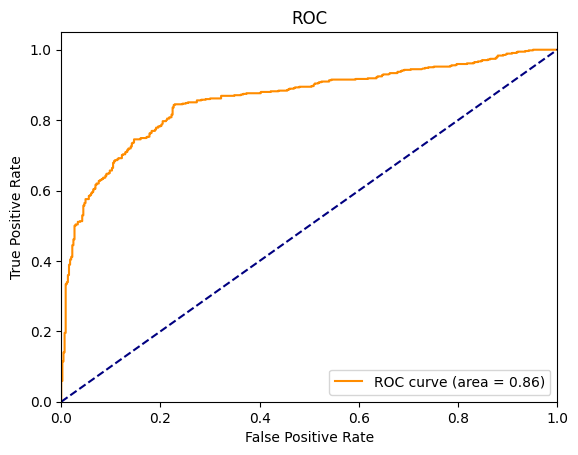
\includegraphics[width=\textwidth, height=6cm]{Figures/balanced_data/less_data/withoutbn/resnet/roc.png}
        \captionsetup{labelformat=empty}
        \caption{Combination 1}
        \label{fig:u_wo_r_roc}
    \end{minipage}
    \hfill
    \begin{minipage}[b]{0.49\textwidth}
        \centering
        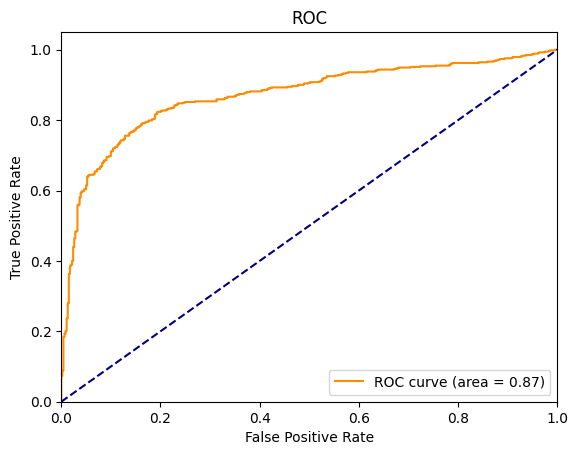
\includegraphics[width=\textwidth, height=6cm]{Figures/balanced_data/less_data/withbn/resnet/roc.png}
        \captionsetup{labelformat=empty}
        \caption{Combination 2}
        \label{fig:u_w_r_roc}
    \end{minipage}
    \captionsetup{labelformat=default}
    \caption{ResNet-50 Area under the ROC Curve}
\end{figure}

\subsubsection{MobileNet V1}


\begin{figure}[H]
    \centering
    \begin{minipage}[b]{0.49\textwidth}
        \centering
        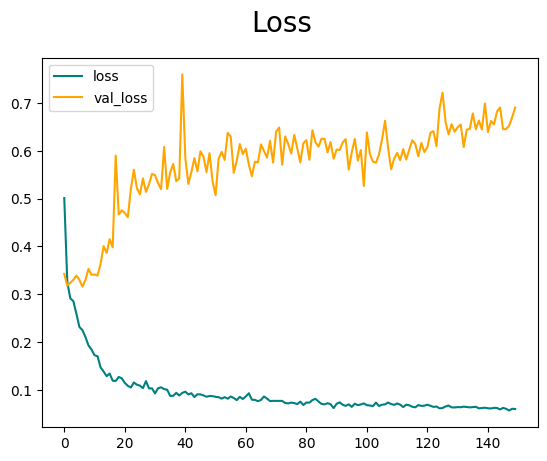
\includegraphics[width=\textwidth, height=6cm]{Figures/balanced_data/less_data/withoutbn/mn1/loss.png}
        \captionsetup{labelformat=empty}
        \caption{Combination 1}
        \label{fig:u_wo_r_l}
    \end{minipage}
    \hfill
    \begin{minipage}[b]{0.49\textwidth}
        \centering
        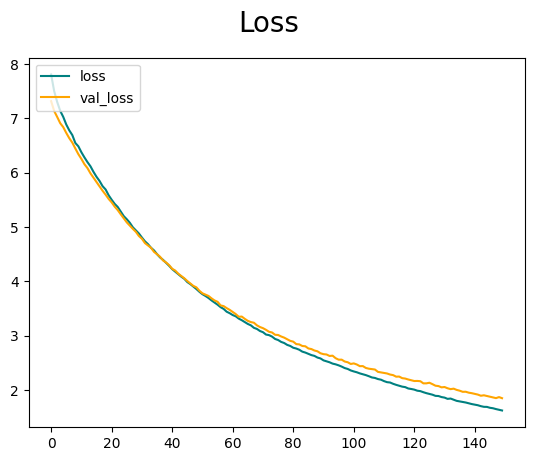
\includegraphics[width=\textwidth, height=6cm]{Figures/balanced_data/less_data/withbn/mn1/loss.png}
        \captionsetup{labelformat=empty}
        \caption{Combination 2}
        \label{fig:u_w_r_l}
    \end{minipage}
    \captionsetup{labelformat=default}
    \caption{MobilNet V1 Loss Curves}
\end{figure}

\begin{figure}[H]
    \centering
    \begin{minipage}[b]{0.49\textwidth}
        \centering
        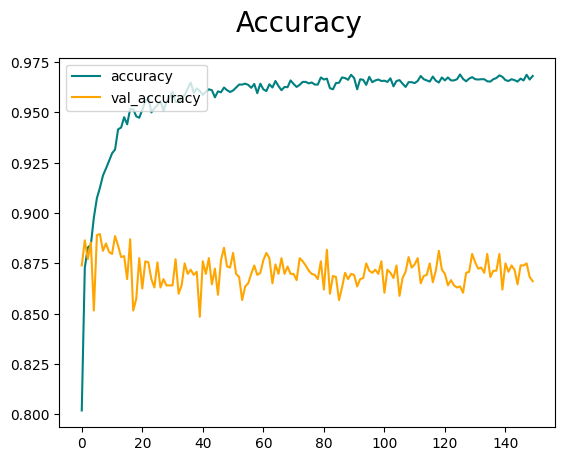
\includegraphics[width=\textwidth, height=6cm]{Figures/balanced_data/less_data/withoutbn/mn1/accuracy.png}
        \captionsetup{labelformat=empty}
        \caption{Combination 1}
        \label{fig:u_wo_r_a}
    \end{minipage}
    \hfill
    \begin{minipage}[b]{0.49\textwidth}
        \centering
        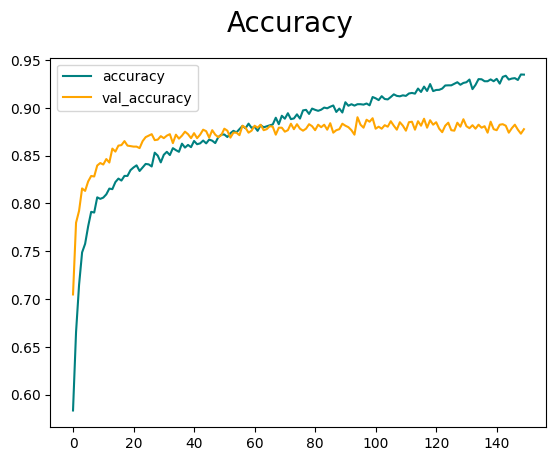
\includegraphics[width=\textwidth, height=6cm]{Figures/balanced_data/less_data/withbn/mn1/accuracy.png}
        \captionsetup{labelformat=empty}
        \caption{Combination 2}
        \label{fig:u_w_r_a}
    \end{minipage}
    \captionsetup{labelformat=default}
    \caption{MobilNet V1 Accuracy Curves}
\end{figure}


\begin{figure}[H]
    \centering
    \begin{minipage}[b]{0.49\textwidth}
        \centering
        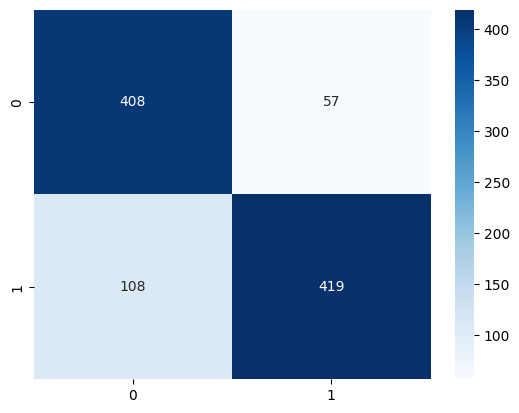
\includegraphics[width=\textwidth, height=6cm]{Figures/balanced_data/less_data/withoutbn/mn1/cm.png}
        \captionsetup{labelformat=empty}
        \caption{Combination 1}
        \label{fig:u_wo_r_cm}
    \end{minipage}
    \hfill
    \begin{minipage}[b]{0.49\textwidth}
        \centering
        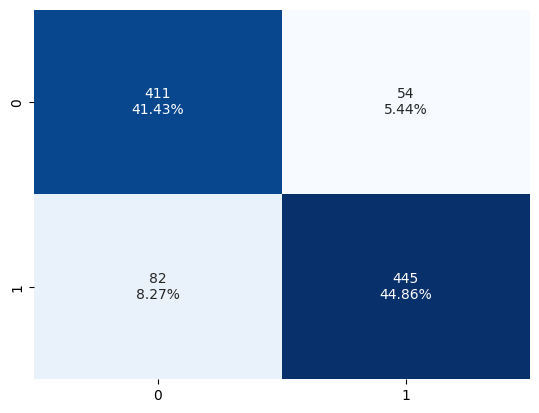
\includegraphics[width=\textwidth, height=6cm]{Figures/balanced_data/less_data/withbn/mn1/cm.png}
        \captionsetup{labelformat=empty}
        \caption{Combination 2}
        \label{fig:u_w_r_cm}
    \end{minipage}
    \captionsetup{labelformat=default}
    \caption{MobilNet V1 Confusion Matrix}
\end{figure}


\begin{figure}[H]
    \centering
    \begin{minipage}[b]{0.49\textwidth}
        \centering
        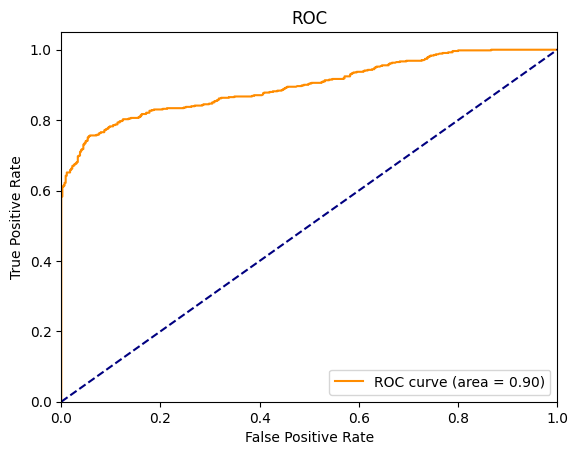
\includegraphics[width=\textwidth, height=6cm]{Figures/balanced_data/less_data/withoutbn/mn1/roc.png}
        \captionsetup{labelformat=empty}
        \caption{Combination 1}
        \label{fig:u_wo_r_roc}
    \end{minipage}
    \hfill
    \begin{minipage}[b]{0.49\textwidth}
        \centering
        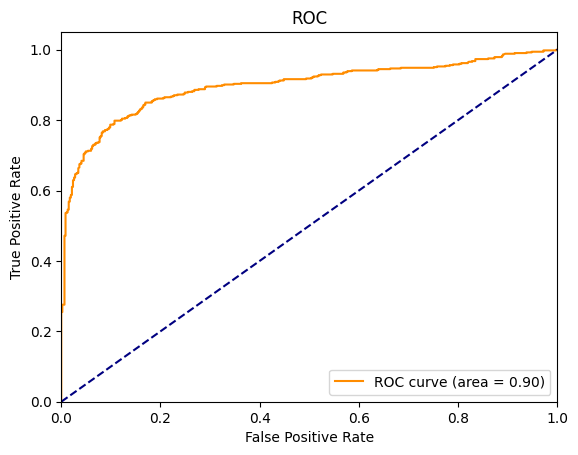
\includegraphics[width=\textwidth, height=6cm]{Figures/balanced_data/less_data/withbn/mn1/roc.png}
        \captionsetup{labelformat=empty}
        \caption{Combination 2}
        \label{fig:u_w_r_roc}
    \end{minipage}
    \captionsetup{labelformat=default}
    \caption{MobilNet V1 Area under the ROC Curve}
\end{figure}

\subsubsection{MobileNet V2}

\begin{figure}[H]
    \centering
    \begin{minipage}[b]{0.49\textwidth}
        \centering
        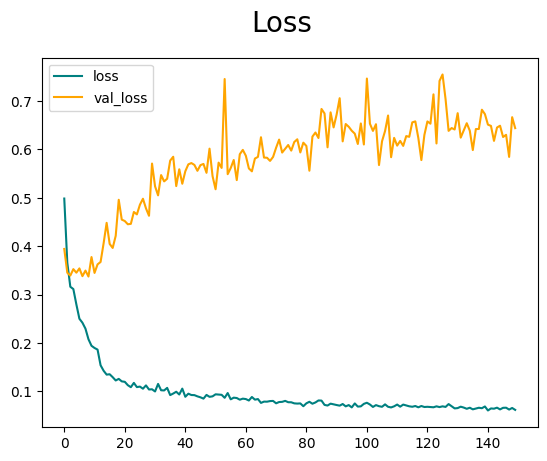
\includegraphics[width=\textwidth, height=6cm]{Figures/balanced_data/less_data/withoutbn/mn2/loss.png}
        \captionsetup{labelformat=empty}
        \caption{Combination 1}
        \label{fig:u_wo_r_l}
    \end{minipage}
    \hfill
    \begin{minipage}[b]{0.49\textwidth}
        \centering
        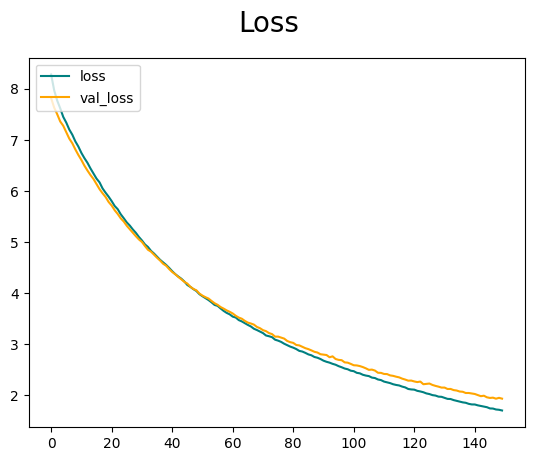
\includegraphics[width=\textwidth, height=6cm]{Figures/balanced_data/less_data/withbn/mn2/loss.png}
        \captionsetup{labelformat=empty}
        \caption{Combination 2}
        \label{fig:u_w_r_l}
    \end{minipage}
    \captionsetup{labelformat=default}
    \caption{MobilNet V2 Loss Curves}
\end{figure}

\begin{figure}[H]
    \centering
    \begin{minipage}[b]{0.49\textwidth}
        \centering
        \includegraphics[width=\textwidth, height=6cm]{Figures/balanced_data/less_data/withoutbn/mn2/accuracy.png}
        \captionsetup{labelformat=empty}
        \caption{Combination 1}
        \label{fig:u_wo_r_a}
    \end{minipage}
    \hfill
    \begin{minipage}[b]{0.49\textwidth}
        \centering
        \includegraphics[width=\textwidth, height=6cm]{Figures/balanced_data/less_data/withbn/mn2/accuracy.png}
        \captionsetup{labelformat=empty}
        \caption{Combination 2}
        \label{fig:u_w_r_a}
    \end{minipage}
    \captionsetup{labelformat=default}
    \caption{MobilNet V2 Accuracy Curves}
\end{figure}


\begin{figure}[H]
    \centering
    \begin{minipage}[b]{0.49\textwidth}
        \centering
        \includegraphics[width=\textwidth, height=6cm]{Figures/balanced_data/less_data/withoutbn/mn2/cm.png}
        \captionsetup{labelformat=empty}
        \caption{Combination 1}
        \label{fig:u_wo_r_cm}
    \end{minipage}
    \hfill
    \begin{minipage}[b]{0.49\textwidth}
        \centering
        \includegraphics[width=\textwidth, height=6cm]{Figures/balanced_data/less_data/withbn/mn2/cm.png}
        \captionsetup{labelformat=empty}
        \caption{Combination 2}
        \label{fig:u_w_r_cm}
    \end{minipage}
    \captionsetup{labelformat=default}
    \caption{MobilNet V2 Confusion Matrix}
\end{figure}

\begin{figure}[H]
    \centering
    \begin{minipage}[b]{0.49\textwidth}
        \centering
        \includegraphics[width=\textwidth, height=6cm]{Figures/balanced_data/less_data/withoutbn/mn2/roc.png}
        \captionsetup{labelformat=empty}
        \caption{Combination 1}
        \label{fig:u_wo_r_roc}
    \end{minipage}
    \hfill
    \begin{minipage}[b]{0.49\textwidth}
        \centering
        \includegraphics[width=\textwidth, height=6cm]{Figures/balanced_data/less_data/withbn/mn2/roc.png}
        \captionsetup{labelformat=empty}
        \caption{Combination 2}
        \label{fig:u_w_r_roc}
    \end{minipage}
    \captionsetup{labelformat=default}
    \caption{MobilNet V2 Area under the ROC Curve}
\end{figure}

\subsubsection{MobileNet V3}

\begin{figure}[H]
    \centering
    \begin{minipage}[b]{0.49\textwidth}
        \centering
        \includegraphics[width=\textwidth, height=6cm]{Figures/balanced_data/less_data/withoutbn/mn3/loss.png}
        \captionsetup{labelformat=empty}
        \caption{Combination 1}
        \label{fig:u_wo_r_l}
    \end{minipage}
    \hfill
    \begin{minipage}[b]{0.49\textwidth}
        \centering
        \includegraphics[width=\textwidth, height=6cm]{Figures/balanced_data/less_data/withbn/mn3/loss.png}
        \captionsetup{labelformat=empty}
        \caption{Combination 2}
        \label{fig:u_w_r_l}
    \end{minipage}
    \captionsetup{labelformat=default}
    \caption{MobilNet V3 Loss Curves}
\end{figure}

\begin{figure}[H]
    \centering
    \begin{minipage}[b]{0.49\textwidth}
        \centering
        \includegraphics[width=\textwidth, height=6cm]{Figures/balanced_data/less_data/withoutbn/mn3/accuracy.png}
        \captionsetup{labelformat=empty}
        \caption{Combination 1}
        \label{fig:u_wo_r_a}
    \end{minipage}
    \hfill
    \begin{minipage}[b]{0.49\textwidth}
        \centering
        \includegraphics[width=\textwidth, height=6cm]{Figures/balanced_data/less_data/withbn/mn3/accuracy.png}
        \captionsetup{labelformat=empty}
        \caption{Combination 2}
        \label{fig:u_w_r_a}
    \end{minipage}
    \captionsetup{labelformat=default}
    \caption{MobilNet V3 Accuracy Curves}
\end{figure}


\begin{figure}[H]
    \centering
    \begin{minipage}[b]{0.49\textwidth}
        \centering
        \includegraphics[width=\textwidth, height=6cm]{Figures/balanced_data/less_data/withoutbn/mn3/cm.png}
        \captionsetup{labelformat=empty}
        \caption{Combination 1}
        \label{fig:u_wo_r_cm}
    \end{minipage}
    \hfill
    \begin{minipage}[b]{0.49\textwidth}
        \centering
        \includegraphics[width=\textwidth, height=6cm]{Figures/balanced_data/less_data/withbn/mn3/cm.png}
        \captionsetup{labelformat=empty}
        \caption{Combination 2}
        \label{fig:u_w_r_cm}
    \end{minipage}
    \captionsetup{labelformat=default}
    \caption{MobilNet V3 Confusion Matrix}
\end{figure}


\begin{figure}[H]
    \centering
    \begin{minipage}[b]{0.49\textwidth}
        \centering
        \includegraphics[width=\textwidth, height=6cm]{Figures/balanced_data/less_data/withoutbn/mn3/roc.png}
        \captionsetup{labelformat=empty}
        \caption{Combination 1}
        \label{fig:u_wo_r_roc}
    \end{minipage}
    \hfill
    \begin{minipage}[b]{0.49\textwidth}
        \centering
        \includegraphics[width=\textwidth, height=6cm]{Figures/balanced_data/less_data/withbn/mn3/roc.png}
        \captionsetup{labelformat=empty}
        \caption{Combination 2}
        \label{fig:u_w_r_roc}
    \end{minipage}
    \captionsetup{labelformat=default}
    \caption{MobilNet V3 Area under the ROC Curve}
\end{figure}

\subsection{With Augmentation}

\begin{table}[H]
\centering
\begin{tabularx}{\textwidth}{@{} *4{X} @{}}
\toprule
\textbf{Label} & \textbf{Class} & \textbf{Images} & \textbf{Distribution}\\
\midrule
    Mature     & 0 & 25612 & 50\%  \\[1.3ex]
    Trout    &  1 & 25270 & 50\% \\[1.3ex]
\bottomrule
\end{tabularx}
\caption{Balanced dataset with data augmentation}
\label{table:data_type3}
\end{table}

\begin{table}[H]
\centering
\begin{tabularx}{\textwidth}{@{} *5{X} @{}}
\toprule
\multicolumn{5}{c}{\textbf{Model Combination Type 1 (\ref{subsubsec:variation_1})}}                                    \\ \midrule
\raggedright \textbf{Model Metrics}           & \textbf{ResNet-50} & \textbf{MobileNet V1} & \textbf{MobileNet V2} & \textbf{MobileNet V3} \\ \midrule
Batch Size           & 64          &   64           &  64            &  64            \\ \midrule
Train Size           & 557          &  557            & 557             &  557             \\  \midrule
Validation Size      & 159          &  159            & 159             &  159            \\ \midrule
Test Size            & 80          &   80           &   80           &  80            \\ \midrule
\raggedright Total Params     &   24,637,826          &  3,754,690            &  2,914,882            &    4,883,330          \\ \midrule
\raggedright Trainable Params &  1,050,114         & 525,826             & 656,898             &   656,898           \\ \midrule
Learning Rate        &   0.001        & 0.001             &  0.001            &  0.001            \\ \midrule
Epochs               &  150         &  150            &  150            &   500           \\ \midrule
Training Time (mins)        & 247          & 158              & 145             &  584            \\ \midrule
\addlinespace
\addlinespace
\midrule
\multicolumn{5}{c}{\textbf{Model Combination Type 2 (\ref{subsubsec:variation_2})}}                                    \\ \midrule
\raggedright \textbf{Model Metrics}           & \textbf{ResNet-50} & \textbf{MobileNet V1} & \textbf{MobileNet V2} & \textbf{MobileNet V3} \\ \midrule
Batch Size           &  64         & 64             &   64           &   64           \\ \midrule
Train Size           &   557        & 557             &  557            &  557            \\  \midrule
Validation Size      &   159        & 159             &  159            &  159            \\ \midrule
Test Size            &  80         &  80            &    80          &   80           \\ \midrule
\raggedright Total Params     &   24,639,874      & 3,756,738             & 2,916,930             &  4,883,330            \\ \midrule
\raggedright Trainable Params &  1,051,138         &  526,850             & 657,922             &  656,898            \\ \midrule
Learning Rate        &  0.00001         & 0.00001             &  0.00001            &   0.0001           \\ \midrule
Epochs               &   150        &  150            &  150            & 1000             \\ \midrule
Training Time (mins)        & 240          &  162            &  144            &  870            \\
\bottomrule
\end{tabularx}
\caption{Model Setup for Combination Type 1 and 2 }
\label{table:results_5}
\end{table}


\begin{table}[H]
\centering
\begin{tabularx}{\textwidth}{@{} *5{X} @{}}
\toprule
\multicolumn{5}{c}{\textbf{Evaluation Metrics}}                                    \\ \midrule
\addlinespace
\raggedright \textbf{Metrics}           & \textbf{ResNet-50} & \textbf{MobileNet V1} & \textbf{MobileNet V2} & \textbf{MobileNet V3} \\ \midrule
\multicolumn{5}{c}{\textbf{Model Combination Type 1 (\ref{subsubsec:variation_1})}}                                    \\ \midrule
Accuracy             &  84.5\%         &  90.5\%            &  89.4\%            & 75.5\%             \\ \midrule
Precision            &  85.1\%         &  91.7\%            &  90.1\%            & 68.2\%             \\ \midrule
Recall               &  82.9\%         &  88.6\%            &  88.1\%            & 93.6\%            \\ \midrule
F1 Score               &  0.83         &  0.89            &  0.89            & 0.79           \\ \midrule
\multicolumn{5}{c}{\textbf{Model Combination Type 2 (\ref{subsubsec:variation_2})}}                                    \\ \midrule
Accuracy             &  80.5\%         &  90.9\%            &  90.6\%            &   79.6\%           \\ \midrule
Precision            &  73.3\%         &  90.5\%            &  89.9\%            &   79.3\%           \\ \midrule
Recall               &  94.3\%         &  91.0\%            &  90.9\%            &   78.7\%          \\ \midrule
F1 Score               &  0.82         &  0.90            &  0.89            &   0.78         \\ 
\bottomrule
\end{tabularx}
\caption{Evaluation Metrics for Model Combinations Type 1 and 2 }
\label{table:results_6}
\end{table}

\subsubsection{ResNet-50}

\begin{figure}[H]
    \centering
    \begin{minipage}[b]{0.49\textwidth}
        \centering
        \includegraphics[width=\textwidth, height=6cm]{Figures/balanced_data/more_data/withoutbn/resnet/loss.png}
        \captionsetup{labelformat=empty}
        \caption{Combination 1}
        \label{fig:u_wo_r_l}
    \end{minipage}
    \hfill
    \begin{minipage}[b]{0.49\textwidth}
        \centering
        \includegraphics[width=\textwidth, height=6cm]{Figures/balanced_data/more_data/withbn/resnet/loss.png}
        \captionsetup{labelformat=empty}
        \caption{Combination 2}
        \label{fig:u_w_r_l}
    \end{minipage}
    \captionsetup{labelformat=default}
    \caption{ResNet-50 Loss Curves}
\end{figure}

\begin{figure}[H]
    \centering
    \begin{minipage}[b]{0.49\textwidth}
        \centering
        \includegraphics[width=\textwidth, height=6cm]{Figures/balanced_data/more_data/withoutbn/resnet/accuracy.png}
        \captionsetup{labelformat=empty}
        \caption{Combination 1}
        \label{fig:u_wo_r_a}
    \end{minipage}
    \hfill
    \begin{minipage}[b]{0.49\textwidth}
        \centering
        \includegraphics[width=\textwidth, height=6cm]{Figures/balanced_data/more_data/withbn/resnet/accuracy.png}
        \captionsetup{labelformat=empty}
        \caption{Combination 2}
        \label{fig:u_w_r_a}
    \end{minipage}
    \captionsetup{labelformat=default}
    \caption{ResNet-50 Accuracy Curves}
\end{figure}


\begin{figure}[H]
    \centering
    \begin{minipage}[b]{0.49\textwidth}
        \centering
        \includegraphics[width=\textwidth, height=6cm]{Figures/balanced_data/more_data/withoutbn/resnet/cm.png}
        \captionsetup{labelformat=empty}
        \caption{Combination 1}
        \label{fig:u_wo_r_cm}
    \end{minipage}
    \hfill
    \begin{minipage}[b]{0.49\textwidth}
        \centering
        \includegraphics[width=\textwidth, height=6cm]{Figures/balanced_data/more_data/withbn/resnet/cm.png}
        \captionsetup{labelformat=empty}
        \caption{Combination 2}
        \label{fig:u_w_r_cm}
    \end{minipage}
    \captionsetup{labelformat=default}
    \caption{ResNet-50 Confusion Matrix}
\end{figure}


\begin{figure}[H]
    \centering
    \begin{minipage}[b]{0.49\textwidth}
        \centering
        \includegraphics[width=\textwidth, height=6cm]{Figures/balanced_data/more_data/withoutbn/resnet/roc.png}
        \captionsetup{labelformat=empty}
        \caption{Combination 1}
        \label{fig:u_wo_r_roc}
    \end{minipage}
    \hfill
    \begin{minipage}[b]{0.49\textwidth}
        \centering
        \includegraphics[width=\textwidth, height=6cm]{Figures/balanced_data/more_data/withbn/resnet/roc.png}
        \captionsetup{labelformat=empty}
        \caption{Combination 2}
        \label{fig:u_w_r_roc}
    \end{minipage}
    \captionsetup{labelformat=default}
    \caption{ResNet-50 Area under the Curve}
\end{figure}

\subsubsection{MobileNet V1}


\begin{figure}[H]
    \centering
    \begin{minipage}[b]{0.49\textwidth}
        \centering
        \includegraphics[width=\textwidth, height=6cm]{Figures/balanced_data/more_data/withoutbn/mn1/loss.png}
        \captionsetup{labelformat=empty}
        \caption{Combination 1}
        \label{fig:u_wo_r_l}
    \end{minipage}
    \hfill
    \begin{minipage}[b]{0.49\textwidth}
        \centering
        \includegraphics[width=\textwidth, height=6cm]{Figures/balanced_data/more_data/withbn/mn1/loss.png}
        \captionsetup{labelformat=empty}
        \caption{Combination 2}
        \label{fig:u_w_r_l}
    \end{minipage}
    \captionsetup{labelformat=default}
    \caption{MobilNet V1 Loss Curves}
\end{figure}

\begin{figure}[H]
    \centering
    \begin{minipage}[b]{0.49\textwidth}
        \centering
        \includegraphics[width=\textwidth, height=6cm]{Figures/balanced_data/more_data/withoutbn/mn1/accuracy.png}
        \captionsetup{labelformat=empty}
        \caption{Combination 1}
        \label{fig:u_wo_r_a}
    \end{minipage}
    \hfill
    \begin{minipage}[b]{0.49\textwidth}
        \centering
        \includegraphics[width=\textwidth, height=6cm]{Figures/balanced_data/more_data/withbn/mn1/accuracy.png}
        \captionsetup{labelformat=empty}
        \caption{Combination 2}
        \label{fig:u_w_r_a}
    \end{minipage}
    \captionsetup{labelformat=default}
    \caption{MobilNet V1 Accuracy Curves}
\end{figure}


\begin{figure}[H]
    \centering
    \begin{minipage}[b]{0.49\textwidth}
        \centering
        \includegraphics[width=\textwidth, height=6cm]{Figures/balanced_data/more_data/withoutbn/mn1/cm.png}
        \captionsetup{labelformat=empty}
        \caption{Combination 1}
        \label{fig:u_wo_r_cm}
    \end{minipage}
    \hfill
    \begin{minipage}[b]{0.49\textwidth}
        \centering
        \includegraphics[width=\textwidth, height=6cm]{Figures/balanced_data/more_data/withbn/mn1/cm.png}
        \captionsetup{labelformat=empty}
        \caption{Combination 2}
        \label{fig:u_w_r_cm}
    \end{minipage}
    \captionsetup{labelformat=default}
    \caption{MobilNet V1 Confusion Matrix}
\end{figure}


\begin{figure}[H]
    \centering
    \begin{minipage}[b]{0.49\textwidth}
        \centering
        \includegraphics[width=\textwidth, height=6cm]{Figures/balanced_data/more_data/withoutbn/mn1/roc.png}
        \captionsetup{labelformat=empty}
        \caption{Combination 1}
        \label{fig:u_wo_r_roc}
    \end{minipage}
    \hfill
    \begin{minipage}[b]{0.49\textwidth}
        \centering
        \includegraphics[width=\textwidth, height=6cm]{Figures/balanced_data/more_data/withbn/mn1/roc.png}
        \captionsetup{labelformat=empty}
        \caption{Combination 2}
        \label{fig:u_w_r_roc}
    \end{minipage}
    \captionsetup{labelformat=default}
    \caption{MobilNet V1 Area under the ROC Curve}
\end{figure}

\subsubsection{MobileNet V2}

\begin{figure}[H]
    \centering
    \begin{minipage}[b]{0.49\textwidth}
        \centering
        \includegraphics[width=\textwidth, height=6cm]{Figures/balanced_data/more_data/withoutbn/mn2/loss.png}
        \captionsetup{labelformat=empty}
        \caption{Combination 1}
        \label{fig:u_wo_r_l}
    \end{minipage}
    \hfill
    \begin{minipage}[b]{0.49\textwidth}
        \centering
        \includegraphics[width=\textwidth, height=6cm]{Figures/balanced_data/more_data/withbn/mn2/loss.png}
        \captionsetup{labelformat=empty}
        \caption{Combination 2}
        \label{fig:u_w_r_l}
    \end{minipage}
    \captionsetup{labelformat=default}
    \caption{MobilNet V2 Loss Curves}
\end{figure}

\begin{figure}[H]
    \centering
    \begin{minipage}[b]{0.49\textwidth}
        \centering
        \includegraphics[width=\textwidth, height=6cm]{Figures/balanced_data/more_data/withoutbn/mn2/accuracy.png}
        \captionsetup{labelformat=empty}
        \caption{Combination 1}
        \label{fig:u_wo_r_a}
    \end{minipage}
    \hfill
    \begin{minipage}[b]{0.49\textwidth}
        \centering
        \includegraphics[width=\textwidth, height=6cm]{Figures/balanced_data/more_data/withbn/mn2/accuracy.png}
        \captionsetup{labelformat=empty}
        \caption{Combination 2}
        \label{fig:u_w_r_a}
    \end{minipage}
    \captionsetup{labelformat=default}
    \caption{MobilNet V2 Accuracy Curves}
\end{figure}


\begin{figure}[H]
    \centering
    \begin{minipage}[b]{0.49\textwidth}
        \centering
        \includegraphics[width=\textwidth, height=6cm]{Figures/balanced_data/more_data/withoutbn/mn2/cm.png}
        \captionsetup{labelformat=empty}
        \caption{Combination 1}
        \label{fig:u_wo_r_cm}
    \end{minipage}
    \hfill
    \begin{minipage}[b]{0.49\textwidth}
        \centering
        \includegraphics[width=\textwidth, height=6cm]{Figures/balanced_data/more_data/withbn/mn2/cm.png}
        \captionsetup{labelformat=empty}
        \caption{Combination 2}
        \label{fig:u_w_r_cm}
    \end{minipage}
    \captionsetup{labelformat=default}
    \caption{MobilNet V2 Confusion Matrix}
\end{figure}



\begin{figure}[H]
    \centering
    \begin{minipage}[b]{0.49\textwidth}
        \centering
        \includegraphics[width=\textwidth, height=6cm]{Figures/balanced_data/more_data/withoutbn/mn2/roc.png}
        \captionsetup{labelformat=empty}
        \caption{Combination 1}
        \label{fig:u_wo_r_roc}
    \end{minipage}
    \hfill
    \begin{minipage}[b]{0.49\textwidth}
        \centering
        \includegraphics[width=\textwidth, height=6cm]{Figures/balanced_data/more_data/withbn/mn2/roc.png}
        \captionsetup{labelformat=empty}
        \caption{Combination 2}
        \label{fig:u_w_r_roc}
    \end{minipage}
    \captionsetup{labelformat=default}
    \caption{MobilNet V2 Area under the ROC Curve}
\end{figure}

\subsubsection{MobileNet V3}

\begin{figure}[H]
    \centering
    \begin{minipage}[b]{0.49\textwidth}
        \centering
        \includegraphics[width=\textwidth, height=6cm]{Figures/balanced_data/more_data/withoutbn/mn3/loss.png}
        \captionsetup{labelformat=empty}
        \caption{Combination 1}
        \label{fig:u_wo_r_l}
    \end{minipage}
    \hfill
    \begin{minipage}[b]{0.49\textwidth}
        \centering
        \includegraphics[width=\textwidth, height=6cm]{Figures/balanced_data/more_data/withbn/mn3/loss.png}
        \captionsetup{labelformat=empty}
        \caption{Combination 2}
        \label{fig:u_w_r_l}
    \end{minipage}
    \captionsetup{labelformat=default}
    \caption{MobilNet V3 Loss Curves}
\end{figure}

\begin{figure}[H]
    \centering
    \begin{minipage}[b]{0.49\textwidth}
        \centering
        \includegraphics[width=\textwidth, height=6cm]{Figures/balanced_data/more_data/withoutbn/mn3/accuracy.png}
        \captionsetup{labelformat=empty}
        \caption{Combination 1}
        \label{fig:u_wo_r_a}
    \end{minipage}
    \hfill
    \begin{minipage}[b]{0.49\textwidth}
        \centering
        \includegraphics[width=\textwidth, height=6cm]{Figures/balanced_data/more_data/withbn/mn3/accuracy.png}
        \captionsetup{labelformat=empty}
        \caption{Combination 2}
        \label{fig:u_w_r_a}
    \end{minipage}
    \captionsetup{labelformat=default}
    \caption{MobilNet V3 Accuracy Curves}
\end{figure}


\begin{figure}[H]
    \centering
    \begin{minipage}[b]{0.49\textwidth}
        \centering
        \includegraphics[width=\textwidth, height=6cm]{Figures/balanced_data/more_data/withoutbn/mn3/cm.png}
        \captionsetup{labelformat=empty}
        \caption{Combination 1}
        \label{fig:u_wo_r_cm}
    \end{minipage}
    \hfill
    \begin{minipage}[b]{0.49\textwidth}
        \centering
        \includegraphics[width=\textwidth, height=6cm]{Figures/balanced_data/more_data/withbn/mn3/cm.png}
        \captionsetup{labelformat=empty}
        \caption{Combination 2}
        \label{fig:u_w_r_cm}
    \end{minipage}
    \captionsetup{labelformat=default}
    \caption{MobilNet V3 Confusion Matrix}
\end{figure}



\begin{figure}[H]
    \centering
    \begin{minipage}[b]{0.49\textwidth}
        \centering
        \includegraphics[width=\textwidth, height=6cm]{Figures/balanced_data/more_data/withoutbn/mn3/roc.png}
        \captionsetup{labelformat=empty}
        \caption{Combination 1}
        \label{fig:u_wo_r_roc}
    \end{minipage}
    \hfill
    \begin{minipage}[b]{0.49\textwidth}
        \centering
        \includegraphics[width=\textwidth, height=6cm]{Figures/balanced_data/more_data/withbn/mn3/roc.png}
        \captionsetup{labelformat=empty}
        \caption{Combination 2}
        \label{fig:u_w_r_roc}
    \end{minipage}
    \captionsetup{labelformat=default}
    \caption{MobilNet V3 Area under the ROC Curve}
\end{figure}